% ===== ANNEXES (numérotées) =====
\annexepaysage[page=1,trim=700bp 30bp 30bp 80bp,clip]{Plan_couvercle_repartiteur.pdf}{Plan du couvercle répartiteur}{planrep}{Plan du couvercle répartiteur : vue de dessus, vue de côté, vue de dessous avec les huit canaux et coupe B-B. Il est présenté dans la partie 3.2.}
\hypertarget{planrep}{}
\annexepaysage[page=1]{Plan_couvercle_bouchon.pdf}{Plan de la pièce COUVERCLE (bouchon et embout)}{planbou}{Plan de la pièce COUVERCLE (bouchon et embout). Il est présenté dans la partie 3.2.}
\hypertarget{planbou}{}
\annexepaysage{Schema_hydraulique_hydroponie.pdf}{Schéma hydraulique de la tour}{hydro}{Schéma hydraulique de la tour : bac unique, pompe de circulation -M1, pompes de dosage -M2 à -M4, sondes -B1 à -B4 et appoint manuel. Il est présenté dans la partie 3.1.}

\clearpage\refstepcounter{annexe}\phantomsection\addcontentsline{toc}{section}{Annexe \theannexe{} : Fiche du régulateur MPPT\ix{19} SLC-MT2024}
{\thispagestyle{empty}\centering{\large\bfseries Annexe \theannexe{} : Fiche du régulateur MPPT\ix{19} SLC-MT2024\par}\vspace{4pt}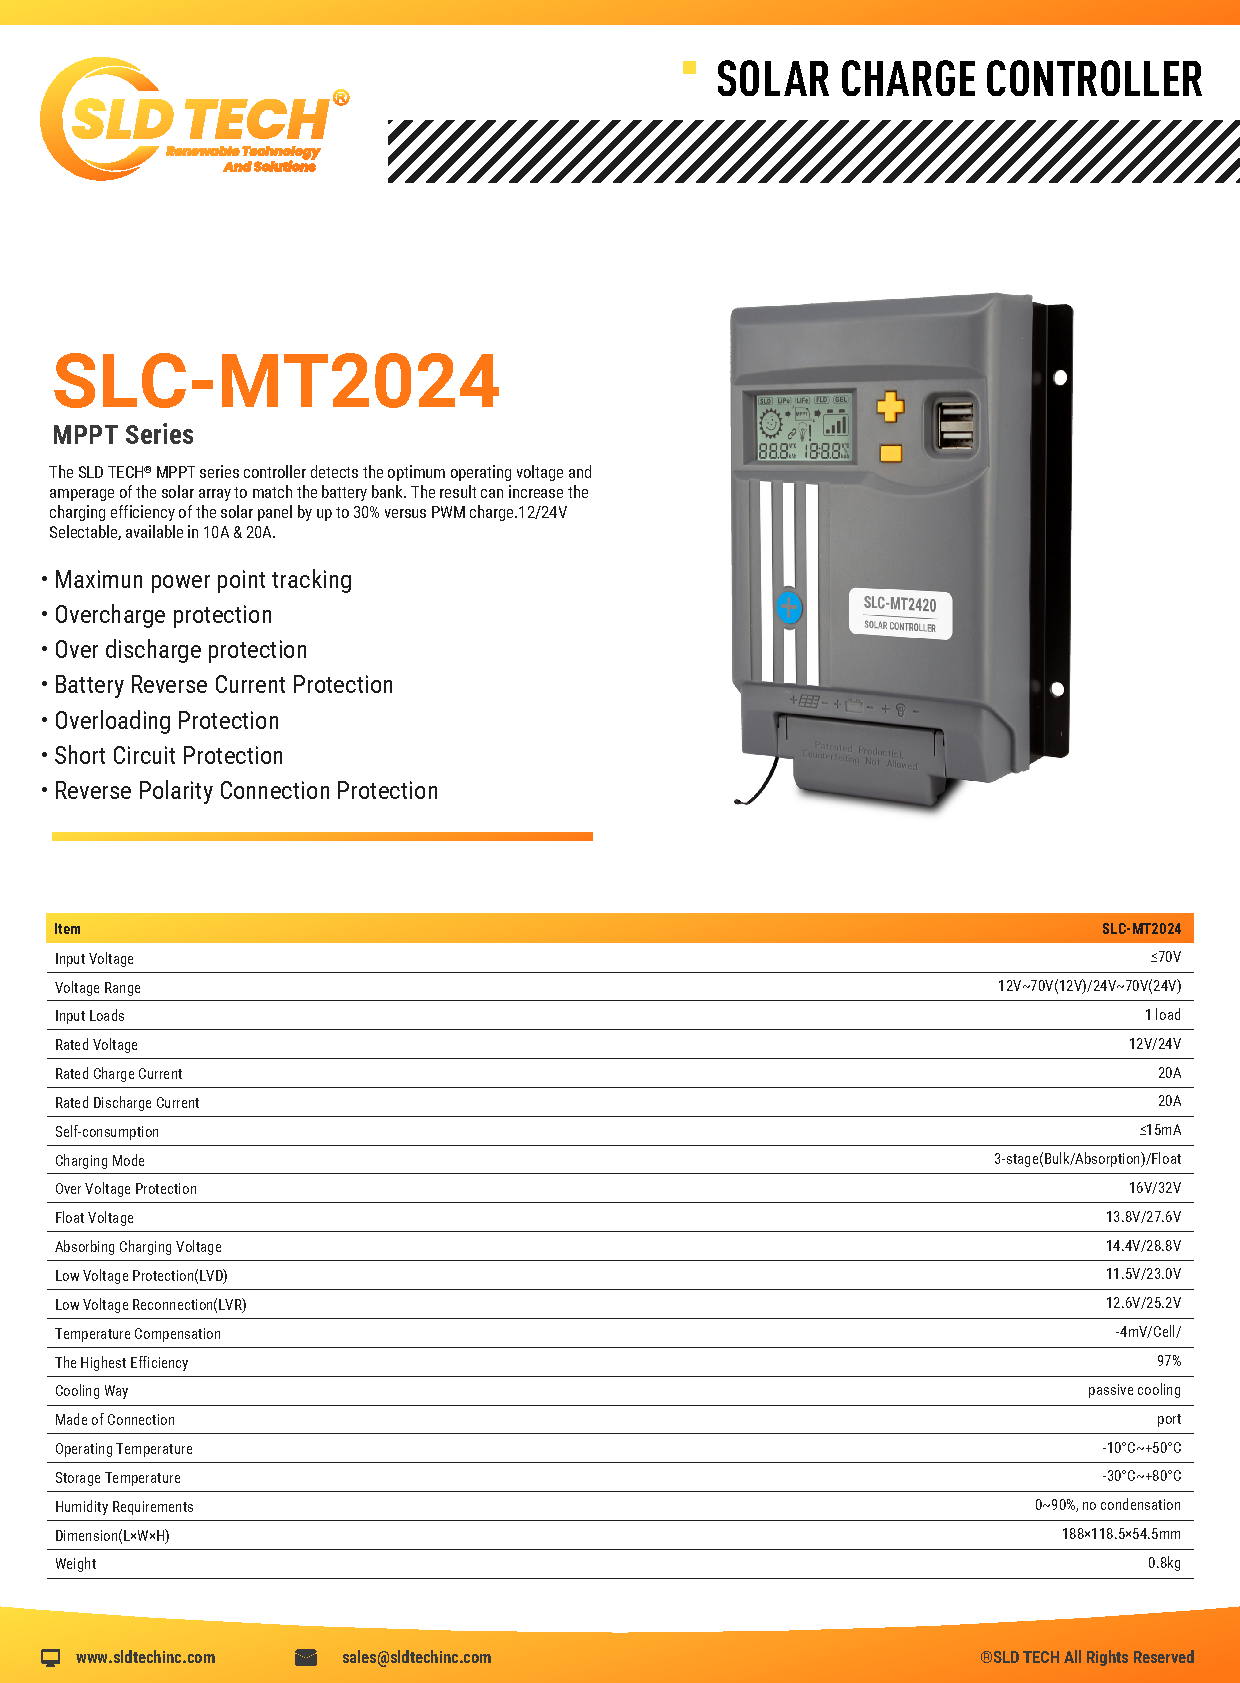
\includegraphics[page=1,width=\textwidth,height=0.86\textheight,keepaspectratio]{SLC-MT2024.pdf}\par}
\clearpage
{\begin{landscape}\thispagestyle{empty}\centering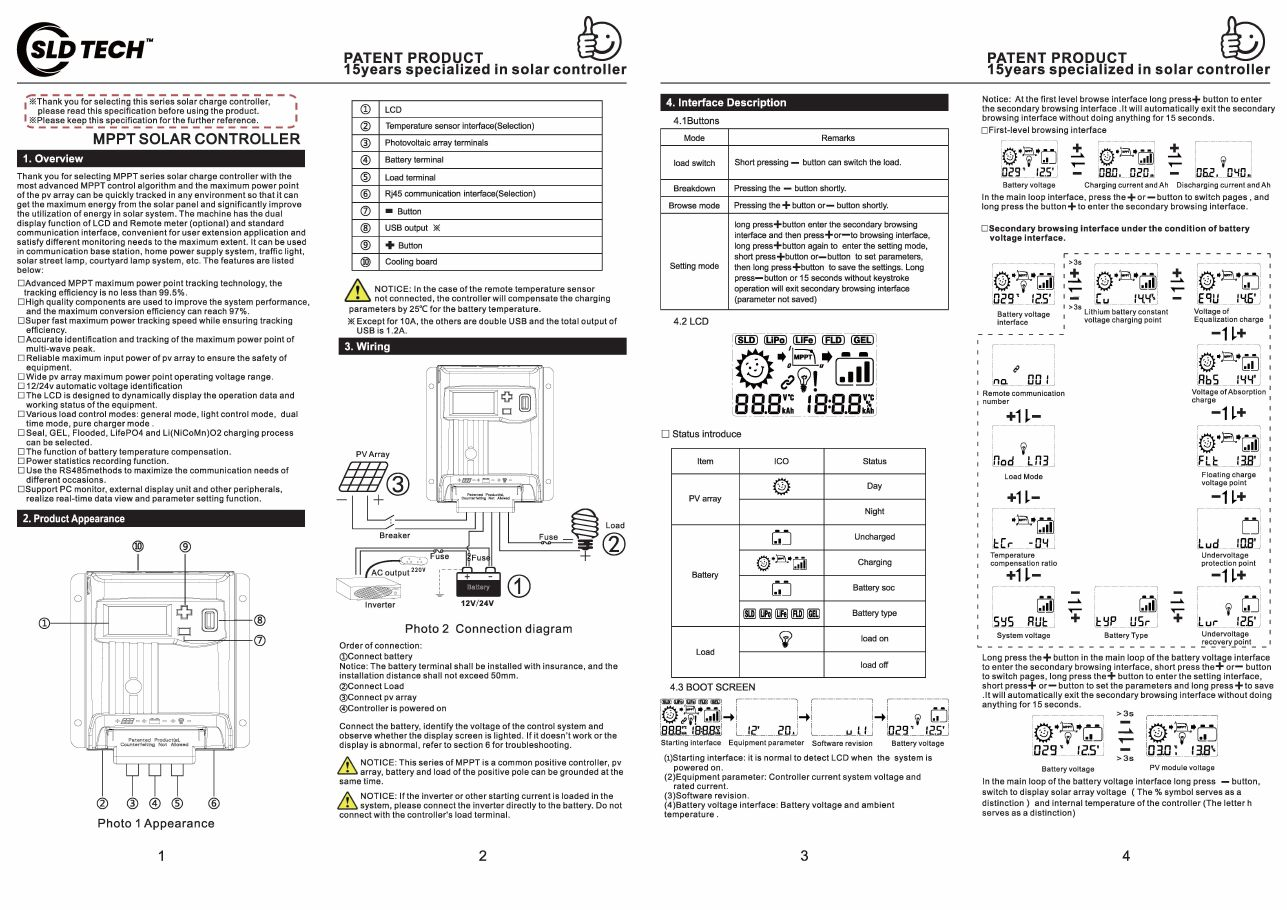
\includegraphics[height=0.93\textwidth,width=0.97\linewidth,keepaspectratio]{img/mppt_manuel_1.jpg}\end{landscape}}
\clearpage
{\begin{landscape}\thispagestyle{empty}\centering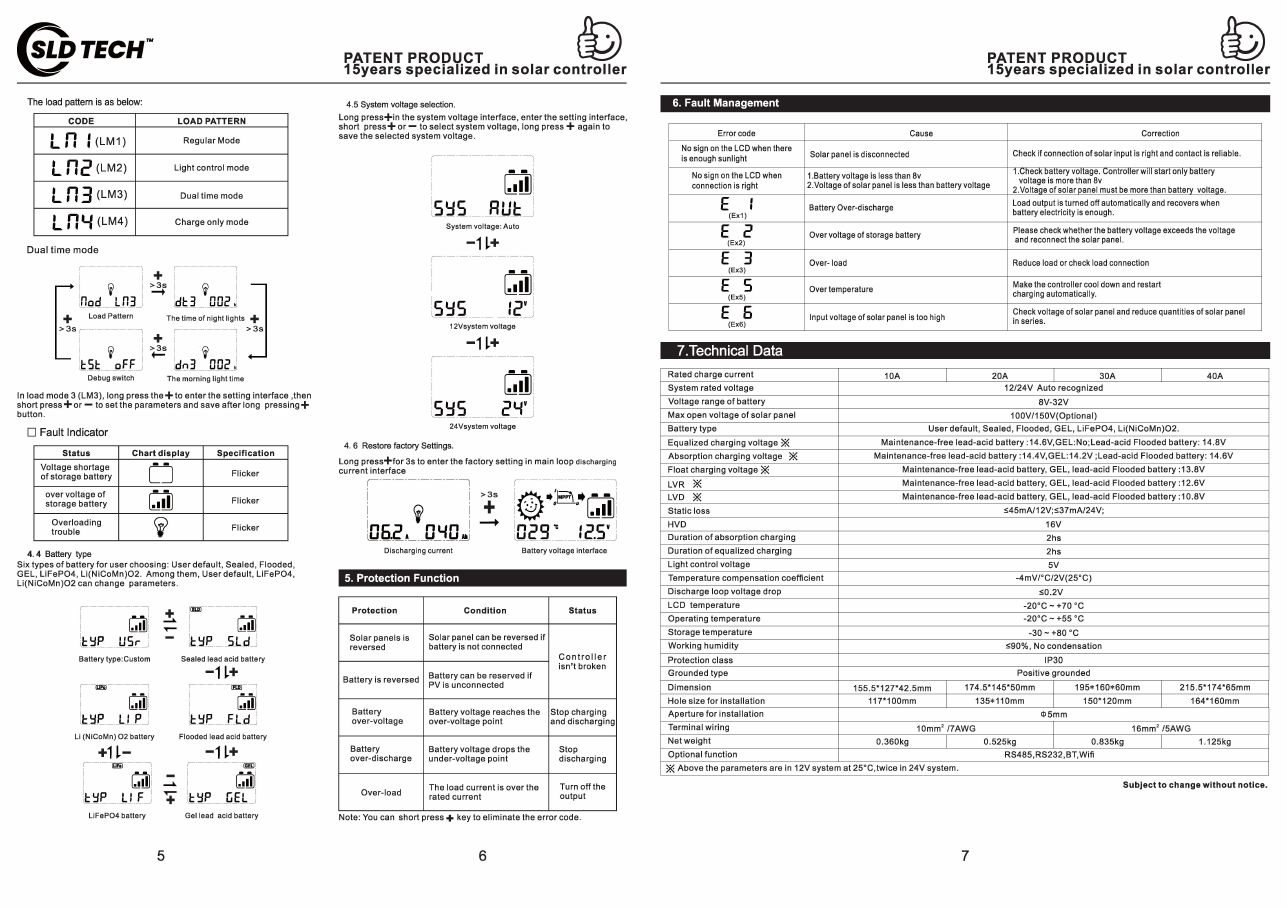
\includegraphics[height=0.93\textwidth,width=0.97\linewidth,keepaspectratio]{img/mppt_manuel_2.jpg}\end{landscape}}

\annexepaysage[page=1]{A000066-schematics.pdf}{Schéma électrique de l'Arduino Uno}{uno1}{Schéma électrique officiel de la carte Arduino Uno Rev3 (référence A000066), publié par le constructeur : alimentation, microcontrôleur et liaison USB. Les noms des broches (D5, D6, A0, A4, A5...) servent de repère pour lire les feuilles de commande de la partie 8.2.}
\pagesuite[page=2]{A000066-schematics.pdf}{uno2}{Schéma électrique officiel de la carte Arduino Uno Rev3 (suite) : les connecteurs.}

% ============================================================
\clearpage
\section*{Fiches techniques du matériel}
\addcontentsline{toc}{section}{Fiches techniques du matériel}

Chaque composant a sa fiche, qui est une annexe numérotée. Elles rassemblent, composant par composant, les caractéristiques utiles à la tour : celles des fiches techniques des fabricants et celles que j'ai relevées sur les pages des revendeurs. Pour chaque composant, je rappelle ensuite ce que la valeur change dans le projet. Les composants sont classés dans l'ordre du tableau de la partie 11 : structure et hydraulique, énergie, calcul et commande, mesures. Une valeur marquée « à mesurer » n'est pas une donnée du fabricant : c'est une hypothèse de mes calculs, à vérifier sur le montage réel.

\Needspace{8\baselineskip}
\subsection*{Structure et hydraulique}

\annexefiche{Tube PVC et bac}
\noindent Le tube est un tube de \qty{1}{m} de diamètre extérieur \qty{159}{mm} et de diamètre intérieur \qty{144}{mm}, dont l'épaisseur de paroi vaut donc :
\[
e = \frac{\qty{159}{mm} - \qty{144}{mm}}{2} = \qty{7,5}{mm}
\]
Le bac fait \qty{152}{L}. Les dimensions du bac et les masses sont des hypothèses de la partie 4, à mesurer.

\annexefiche{Pompe de circulation LPFIDI}
\noindent
\begin{table}[H]
\centering
\begin{tabularx}{\linewidth}{lY}
\hline
Caractéristique & Valeur \\
\hline
Tension d'alimentation & \qty{12}{V} continu \\
Puissance & \qty{19}{W} \\
Courant maximal & \qty{1}{A} \\
Débit maximal & \qty{800}{L/h} \\
Hauteur manométrique maximale & \qty{5}{m} \\
Sortie & filetage mâle 1/2 pouce \\
Câble & très court (rallonge à prévoir) \\
\hline
\end{tabularx}
\end{table}
Le point de fonctionnement réel de la tour est de \qty{388}{L/h} pour une hauteur de \qty{2,57}{m} (partie 3) : la pompe travaille donc bien en dessous de son débit maximal.

\Needspace{8\baselineskip}
\subsection*{Énergie}

\annexefiche{Panneau TE1250 (120 W crête)}
\noindent
\begin{table}[H]
\centering
\begin{tabularx}{\linewidth}{lY}
\hline
Caractéristique & Valeur \\
\hline
Puissance crête $P_c$ & \qty{120}{W} \\
Puissance minimale & \qty{117,5}{W} \\
Tension au point de puissance max $V_{mp}$ & \qty{17,6}{V} \\
Courant au point de puissance max $I_{mp}$ & \qty{6,8}{A} \\
Courant de court-circuit $I_{sc}$ & \qty{7,3}{A} \\
Tension à vide $V_{oc}$ & \qty{22,0}{V} \\
Fusible série maximal & \qty{10}{A} \\
NOCT & \qty{47}{\celsius} \\
\hline
\end{tabularx}
\end{table}
Les coefficients de température que j'utilise (tension $-\qty{80}{mV/\celsius}$, courant $+\qty{0,065}{\percent/\celsius}$, puissance $-\qty{0,5}{\percent/\celsius}$) sont ceux d'un panneau voisin : ce sont des hypothèses. Vérification de la cohérence de la puissance crête :
\begin{align*}
P_{mp} &= V_{mp} \times I_{mp}\\
P_{mp} &= \qty{17,6}{V} \times \qty{6,8}{A}\\
P_{mp} &= \qty{119,68}{W} \approx \qty{120}{W}
\end{align*}

\annexefiche{Régulateur MPPT SLC-MT2024}
\noindent
\begin{table}[H]
\centering
\begin{tabularx}{\linewidth}{lY}
\hline
Caractéristique & Valeur \\
\hline
Tension nominale batterie & \qty{12}{V} ou \qty{24}{V} (détection) \\
Tension d'entrée maximale & \qty{70}{V} \\
Courant de charge / de décharge & \qty{20}{A} / \qty{20}{A} \\
Sortie charge & 1 \\
Autoconsommation & $\leq \qty{15}{mA}$ \\
Charge & 3 étages \\
Absorption / floating & \qty{14,4}{V} / \qty{13,8}{V} \\
Coupure basse (LVD) / reconnexion (LVR) & \qty{11,5}{V} / \qty{12,6}{V} \\
Compensation en température & $-\qty{4}{mV}$ par élément \\
Rendement maximal & \qty{97}{\percent} \\
Refroidissement & passif \\
Température de service & \qtyrange{-10}{50}{\celsius} \\
Dimensions & \qtyproduct{188 x 118,5 x 54,5}{mm} \\
Masse & \qty{0,8}{kg} \\
\hline
\end{tabularx}
\end{table}
La coupure basse à \qty{11,5}{V} protège la batterie plomb d'une décharge profonde ; je m'en sers dans le bilan d'autonomie.

\annexefiche{Batteries au plomb}
\noindent
\begin{table}[H]
\centering
\begin{tabularx}{\linewidth}{lYY}
\hline
Caractéristique & Yuasa NP17-12I & Steco YTX7A-BS \\
\hline
Technologie & plomb étanche à soupape (VRLA, AGM) & sans entretien (AGM supposée) \\
Tension nominale & \qty{12}{V} & \qty{12}{V} \\
Capacité & \qty{17}{Ah} (20 h, jusqu'à \qty{10,5}{V}) & \qty{6}{Ah} \\
Capacité à 10 h & \qty{15,7}{Ah} (jusqu'à \qty{10,8}{V}) & non relevée \\
Dimensions (L x l x h) & \qtyproduct{181 x 76 x 167}{mm} & à relever sur l'étiquette \\
Masse & \qty{6,1}{kg} & à relever \\
Bornes & M5 femelles & à relever \\
Température de service & \qtyrange{-15}{50}{\celsius} (revendeur) & non relevée \\
\hline
\end{tabularx}
\end{table}
Le courant de décharge sur 20 h de la Yuasa se déduit de sa capacité :
\begin{align*}
I_{20} &= \frac{C_{20}}{t}\\
I_{20} &= \frac{\qty{17}{Ah}}{\qty{20}{h}}\\
I_{20} &= \qty{0,85}{A}
\end{align*}
L'énergie nominale des deux batteries mises en parallèle vaut :
\begin{align*}
E &= U \times (C_1 + C_2)\\
E &= \qty{12}{V} \times (\qty{17}{Ah} + \qty{6}{Ah})\\
E &= \qty{276}{Wh}
\end{align*}
Ce chiffre est l'énergie brute ; l'énergie utilisable (\qty{138}{Wh}) tient compte d'une profondeur de décharge de \qty{50}{\percent}, voir partie 5. Avant de mettre la Steco en parallèle avec la Yuasa, je dois lire son étiquette pour confirmer qu'elle est bien de technologie AGM.

\Needspace{8\baselineskip}
\subsection*{Calcul et commande}

\annexefiche{Raspberry Pi 3 Model B}
\noindent
\begin{table}[H]
\centering
\begin{tabularx}{\linewidth}{lY}
\hline
Caractéristique & Valeur \\
\hline
Processeur & Broadcom BCM2837, 4 c\oe urs ARM Cortex-A53, \qty{1,2}{GHz} \\
Mémoire & \qty{1}{Go} LPDDR2 \\
Réseau & Wi-Fi 2,4 GHz, Bluetooth 4.1, Ethernet \\
USB & 4 ports USB 2.0 \\
GPIO & 40 broches, logique \qty{3,3}{V} \\
Alimentation & \qty{5}{V} par micro-USB, \qty{2,5}{A} conseillé \\
Stockage & carte micro-SD \\
\hline
\end{tabularx}
\end{table}
Le Pi tourne en \qty{5}{V} : il passe par le convertisseur \qty{12}{V} vers \qty{5}{V} de la partie 5. Ces valeurs sont celles de la fiche du constructeur.

\annexefiche{Arduino Uno R3}
\noindent
\begin{table}[H]
\centering
\begin{tabularx}{\linewidth}{lY}
\hline
Caractéristique & Valeur \\
\hline
Microcontrôleur & ATmega328P \\
Tension de fonctionnement & \qty{5}{V} \\
Entrées analogiques & 6, convertisseur 10 bits \\
Entrées/sorties numériques & 14 (dont 6 PWM) \\
Mémoire flash / SRAM / EEPROM & \qty{32}{ko} / \qty{2}{ko} / \qty{1}{ko} \\
Fréquence d'horloge & \qty{16}{MHz} \\
Courant maximal par broche & \qty{20}{mA} (conseillé) \\
\hline
\end{tabularx}
\end{table}
La résolution de son convertisseur 10 bits sur \qty{5}{V} se démontre ainsi : il découpe la plage en $2^{10}$ pas.
\begin{align*}
N &= 2^{10} = 1024\\
q &= \frac{\qty{5}{V}}{1024}\\
q &\approx \qty{4,88}{mV}
\end{align*}
C'est trop grossier pour la sonde pH, d'où l'ADS1115\ix{16} plus bas.

\annexefiche{Arduino Sensor Kit (Vittascience)}
\noindent Le kit est une extension à poser sur la carte Uno, qui regroupe 10 modules Grove câblés sur la carte imprimée : voyant, bouton, potentiomètre, buzzer, capteurs de température et d'humidité, de lumière, de son, de pression atmosphérique, accéléromètre et écran OLED. Je n'en utilise que quatre : le capteur de température et d'humidité (DHT20\ix{24}), le capteur de lumière, l'accéléromètre LIS3DHTR (mesure d'inclinaison de la tour) et la prise Grove pour le module d'horloge.

\annexefiche{Horloge temps réel Grove (DS1307)}
\noindent Cette horloge à pile (Grove, DS1307, adresse I2C\ix{12} 0x68) est celle du montage (repère -K4, partie 8.2).

\noindent
\begin{table}[H]
\centering
\begin{tabularx}{\linewidth}{lY}
\hline
Caractéristique & Valeur \\
\hline
Circuit & DS1307, interface I2C\ix{12}, adresse 0x68 \\
Alimentation & \qty{5}{V}, pile bouton CR1225 de secours \\
Information & secondes, minutes, heures, date, mois, année \\
\hline
\end{tabularx}
\end{table}
Valeurs relevées dans la fiche du circuit.

\Needspace{8\baselineskip}
\subsection*{Cartes d'interface à commander}

\annexefiche{Pompe péristaltique 12 V (doseuse)}
\noindent
\begin{table}[H]
\centering
\begin{tabularx}{\linewidth}{lY}
\hline
Caractéristique & Valeur \\
\hline
Tension du moteur & \qty{12}{V} continu \\
Courant du moteur & \qtyrange{200}{300}{mA} \\
Débit maximal & \qty{100}{mL/min} \\
Température de service & \qtyrange{0}{40}{\celsius} \\
Tuyau fourni & silicone, environ \qty{4}{mm} extérieur et \qty{2}{mm} intérieur (la cote varie selon les lots) \\
Masse & \qty{200}{g} \\
Dimensions & moteur \qty{27}{mm} de diamètre, longueur environ \qty{72}{mm} \\
Amorçage & auto-amorçante jusqu'à environ \qty{0,5}{m} \\
Sens de rotation & réversible \\
\hline
\end{tabularx}
\end{table}
Mon calcul de dose utilise un débit de \qty{80}{mL/min} (à mesurer), inférieur au maximum du fabricant. Le volume dosé pendant $t$ vaut :
\begin{align*}
Q &= \frac{\qty{80}{mL}}{\qty{60}{s}} \approx \qty{1,33}{mL/s}\\
V &= Q \times t\\
V &= \qty{1,33}{mL/s} \times \qty{3}{s}\\
V &\approx \qty{4}{mL}
\end{align*}
La puissance électrique de chaque pompe, au courant maximal, vaut :
\begin{align*}
P &= U \times I\\
P &= \qty{12}{V} \times \qty{0,3}{A}\\
P &= \qty{3,6}{W}
\end{align*}

\annexefiche{Tuyau silicone et flexible}
\noindent Le tuyau silicone d'un mètre prolonge celui de la pompe. Il n'est pas de qualité alimentaire garantie : le fabricant le destine aux essais, et il doit être nettoyé avant usage. Le flexible de répartition a un diamètre intérieur de \qty{9}{mm} (mesure faite sur le montage).

\annexefiche{Carte 8 canaux MOSFET (Adafruit 6318)}
\noindent
\begin{table}[H]
\centering
\begin{tabularx}{\linewidth}{lY}
\hline
Caractéristique & Valeur \\
\hline
Expandeur & MCP23017, I2C\ix{12}, adresse par défaut 0x20 \\
Canaux & 8, chacun avec un MOSFET\ix{15} AO3406 canal N et une diode de roue libre \\
Tension de charge & \qtyrange{3}{24}{V} continu \\
Courant par canal & \qty{3,6}{A} en pointe \\
Tension drain-source maximale & \qty{30}{V} \\
Résistance à l'état passant $R_{DS(on)}$ & \qty{70}{m\ohm} \\
Alimentation et logique & \qty{3}{V} ou \qty{5}{V} \\
Dimensions & \qtyproduct{51 x 28 x 10,2}{mm} \\
Masse & \qty{10,7}{g} \\
Chaînage & jusqu'à 8 cartes sur le même bus (3 broches d'adresse) \\
\hline
\end{tabularx}
\end{table}
La perte par effet Joule dans un canal traversé par une pompe de \qty{0,3}{A} vaut :
\begin{align*}
P_{pertes} &= R_{DS(on)} \times I^2\\
P_{pertes} &= \qty{0,070}{\ohm} \times (\qty{0,3}{A})^2\\
P_{pertes} &= \qty{6,3}{mW}
\end{align*}
Elle est négligeable devant la puissance de la pompe.

\annexefiche{Convertisseur ADS1115 (Adafruit)}
\noindent
\begin{table}[H]
\centering
\begin{tabularx}{\linewidth}{lY}
\hline
Caractéristique & Valeur \\
\hline
Résolution & 16 bits \\
Voies & 4 asymétriques ou 2 différentielles \\
Cadence & \qtyrange{8}{860}{échantillons/s} \\
Amplificateur à gain programmable & $\times 2/3$, 1, 2, 4, 8, 16 \\
Alimentation & \qtyrange{2}{5,5}{V} \\
Courant en conversion continue & environ \qty{150}{\micro A} \\
Adresses I2C\ix{12} & 0x48 à 0x4B (4 cartes sur un bus) \\
\hline
\end{tabularx}
\end{table}
Au gain 1, la pleine échelle vaut $\pm\qty{4,096}{V}$ ; en mode asymétrique, le bit de signe est inutilisé et il reste 15 bits utiles, soit $2^{15}$ pas pour \qty{4,096}{V} :
\begin{align*}
q &= \frac{\qty{4,096}{V}}{2^{15}}\\
q &= \frac{\qty{4,096}{V}}{32768}\\
q &= \qty{0,125}{mV}
\end{align*}
Le pas est donc environ 39 fois plus fin que celui du convertisseur de l'Uno :
\[
\frac{\qty{4,88}{mV}}{\qty{0,125}{mV}} \approx 39
\]

\annexefiche{Capteur de niveau eTape (30 cm)}
\noindent
\begin{table}[H]
\centering
\begin{tabularx}{\linewidth}{lY}
\hline
Caractéristique & Valeur \\
\hline
Principe & ruban résistif comprimé par la pression hydrostatique \\
Longueur du capteur (modèle 12") & environ \qty{305}{mm} utiles \\
Gradient de résistance & environ \qty{60}{\ohm/cm} (\qty{150}{\ohm}/pouce) \\
Plage de sortie & \qtyrange{400}{2000}{\ohm}, $\pm\qty{20}{\percent}$ \\
Résistance de référence & \qty{2000}{\ohm} $\pm\qty{20}{\percent}$ \\
Profondeur d'actionnement & environ \qty{25,4}{mm} \\
Puissance maximale & \qty{0,5}{W} \\
Résolution annoncée & \qty{0,25}{mm} \\
Température de service & \qtyrange{-9}{60}{\celsius} \\
Tension d'alimentation du montage & \qty{3}{V} ou \qty{5}{V} \\
\hline
\end{tabularx}
\end{table}
Plus le niveau est bas, plus la résistance est grande. Avec une résistance série $R_s = \qty{560}{\ohm}$ et une alimentation $U_{cc}$, le capteur de résistance $R_e$ forme un diviseur, et la tension mesurée $U_m$ entre la résistance série et la masse se déduit de la loi des mailles :
\begin{align*}
U_{cc} &= (R_s + R_e) \times I\\
U_m &= R_s \times I\\
\frac{U_m}{U_{cc}} &= \frac{R_s}{R_s + R_e}\\
R_e &= R_s \times \left(\frac{U_{cc}}{U_m} - 1\right)
\end{align*}
Avec $U_{cc} = \qty{5}{V}$ et $U_m = \qty{2,5}{V}$, on trouve $R_e = \qty{560}{\ohm}$.

\annexefiche{Capteur de courant et tension INA260 (Adafruit)}
\noindent
\begin{table}[H]
\centering
\begin{tabularx}{\linewidth}{lY}
\hline
Caractéristique & Valeur \\
\hline
Tension de bus mesurable & \qtyrange{0}{36}{V} \\
Courant & $\pm\qty{15}{A}$ en continu \\
Résistance de mesure intégrée & \qty{2}{m\ohm} \\
Erreur de gain & \qty{0,15}{\percent} au maximum \\
Erreur de décalage & \qty{5}{mA} au maximum \\
Alimentation & \qtyrange{2,7}{5,5}{V} \\
Interface & I2C\ix{12}, calcul de la puissance intégré \\
Résolution du courant & environ \qty{1,25}{mA} \\
Montage & côté positif ou côté masse \\
\hline
\end{tabularx}
\end{table}
La chute de tension dans la résistance intégrée, au courant maximal de la charge :
\begin{align*}
\Delta U &= R \times I\\
\Delta U &= \qty{0,002}{\ohm} \times \qty{15}{A}\\
\Delta U &= \qty{30}{mV}
\end{align*}
Au courant du panneau (\qty{6,8}{A}), elle tombe à \qty{13,6}{mV}, négligeable devant \qty{12}{V}.

\annexefiche{Sonde de température DS18B20 étanche}
\noindent
\begin{table}[H]
\centering
\begin{tabularx}{\linewidth}{lY}
\hline
Caractéristique & Valeur \\
\hline
Plage de mesure & \qtyrange{-55}{125}{\celsius} \\
Exactitude & $\pm\qty{0,5}{\celsius}$ de \qtyrange{-10}{85}{\celsius} \\
Résolution & 9 à 12 bits, soit \qty{0,0625}{\celsius} à 12 bits \\
Alimentation & \qtyrange{3}{5,5}{V} \\
Bus & 1-Wire, résistance de rappel \qty{4,7}{k\ohm} \\
Temps de conversion à 12 bits & environ \qty{750}{ms} \\
\hline
\end{tabularx}
\end{table}
À 12 bits, la valeur est codée avec 4 bits après la virgule, donc \qty{1}{\celsius} occupe $2^4 = 16$ pas, d'où :
\[
q = \frac{\qty{1}{\celsius}}{16} = \qty{0,0625}{\celsius}
\]

\annexefiche{Convertisseur 12 V vers 5 V (UBEC)}
\noindent Il alimente le Raspberry Pi et l'Arduino à partir de la batterie. Je prends un modèle de courant de sortie d'au moins \qty{3}{A} : le Pi demande \qty{2,5}{A} au maximum, l'Uno quelques dizaines de milliampères. La puissance dissipée se déduit du rendement $\eta$ (hypothèse : \qty{90}{\percent}) :
\begin{align*}
P_{pertes} &= P_{sortie} \times \left(\frac{1}{\eta} - 1\right)\\
P_{pertes} &= (\qty{5}{V} \times \qty{2,5}{A}) \times \left(\frac{1}{0,9} - 1\right)\\
P_{pertes} &= \qty{12,5}{W} \times 0,111\\
P_{pertes} &\approx \qty{1,4}{W}
\end{align*}

\Needspace{8\baselineskip}
\subsection*{Sondes de mesure}

\annexefiche{Sonde pH Gravity SEN0161-V2 (DFRobot)}
\noindent
\begin{table}[H]
\centering
\begin{tabularx}{\linewidth}{lY}
\hline
Caractéristique & Valeur \\
\hline
Plage de mesure & pH 0 à 14 \\
Exactitude & $\pm0,1$ pH à \qty{25}{\celsius} \\
Température de service & \qtyrange{5}{60}{\celsius} \\
Point zéro & pH $7 \pm 0,5$ \\
Temps de réponse & moins de 2 min \\
Résistance interne & moins de \qty{250}{M\ohm} \\
Durée de vie de la sonde & plus de 0,5 an (selon l'usage) \\
Câble & \qty{100}{cm} \\
Alimentation de la carte & \qtyrange{3,3}{5,5}{V} \\
Tension de sortie & \qtyrange{0}{3,0}{V} analogique \\
Connecteurs & BNC (sonde) et Gravity 3 broches (signal) \\
Étalonnage & deux points, pH 4,0 et pH 7,0 \\
\hline
\end{tabularx}
\end{table}
Le fabricant recommande une compensation de température avec une sonde de type DS18B20\ix{24}, ce que fait ma chaîne de mesure. La sonde ne doit pas rester branchée hors tension longtemps, et se conserve dans sa solution de stockage.

\annexefiche{Sonde de conductivité (sonde fabriquée en graphite)}
\noindent Cette sonde est décrite en détail dans l'étude de la sonde de conductivité (partie 7). Elle est alimentée en courant alternatif par les broches D5 et D6 de l'Arduino, pour limiter l'électrolyse, et lue sur l'entrée A0. La sonde du commerce DFR0300 ne sert plus que de solution de repli.

\annexefiche{Autres capteurs du kit Grove}
\noindent Le DHT20\ix{24} du Sensor Kit mesure l'humidité relative et la température de l'air, sur le bus I2C\ix{12} (adresse 0x38, partie 8.2). La première version du montage utilisait un DHT11 sur la broche D3. Le capteur de lumière est lu sur l'entrée analogique A3. L'accéléromètre LIS3DHTR est sur le bus I2C\ix{12}, à l'adresse 0x19. La clé Wi-Fi USB branchée sur le Raspberry Pi permet l'envoi des mesures au tableau de bord en cas de besoin d'un second réseau.

\annexefiche{Bibliothèques Arduino utilisées}
\noindent Le programme de l'actionneur s'appuie sur Adafruit MCP23017 (2.3.2), Adafruit BusIO (1.17.4), Adafruit ADS1X15 (2.6.2), OneWire (2.3.8), DallasTemperature (4.0.6), DHT sensor library (1.4.7), Adafruit Unified Sensor (1.1.15) et Grove LIS3DHTR (1.2.4).

\annexefiche{Brochage de l'Uno}
\noindent
\begin{table}[H]
\centering
\begin{tabularx}{\linewidth}{lY}
\hline
Broche & Fonction \\
\hline
A1 & signal de la sonde pH (lecture directe, montage provisoire ; ADS1115\ix{16} A0 ensuite) \\
A3 & capteur de lumière \\
D5 / D6 & courant alternatif de la sonde de conductivité fabriquée (lecture sur A0) \\
D2 & bus 1-Wire du DS18B20\ix{24} \\
A4 / A5 & bus I2C\ix{12} (SDA\ix{13} / SCL\ix{14}) : MCP23017, ADS1115\ix{16}, INA260\ix{22}, DS1307, DHT20\ix{24}, BMP280, écran OLED, LIS3DHTR \\
\hline
\end{tabularx}
\end{table}

